\section{Типовые математические схемы}

В практике моделирования на первоначальных этапах формализации объекта используют так называемые \textbf{типовые математические схемы}, к которым относят такие хорошо разраотанные математические объекты, как дифференциальные уравнения, конечные и вероятностные автоматы, системы массового обслуживания и т.д.

\begin{table}[H]
    \centering
    \caption{Типовые математические схемы}
    \label{tab:label}
    \begin{tabular}{|l|l|l|l|}
        \hline
        № & Процесс функционирования & Типовая математическая & Обозначение \\
          & системы & схема & \\
        \hline
        1 & Непрерывно-детерминированный & Дифф. ур-ния & $D$ \\
          & подход & & \\
        \hline
        2 & Дискретно-детерминированный & Конечные автоматы & $F$ \\
          & подход & & \\
        \hline
        3 & Дискретно-стахостический & Вероятностный автомат & $P$ \\
          & подход & & \\
        \hline
        4 & Непрерывно-стахостический процесс & Система массового & $Q$ \\
          & процесс & обслуживания & \\
        \hline
        5 & Обобщенный (универсальный) & Агрегативные системы & $A$ \\
          & процесс & & \\
        \hline
    \end{tabular}
\end{table}

\begin{figure}[H]
    \centering
    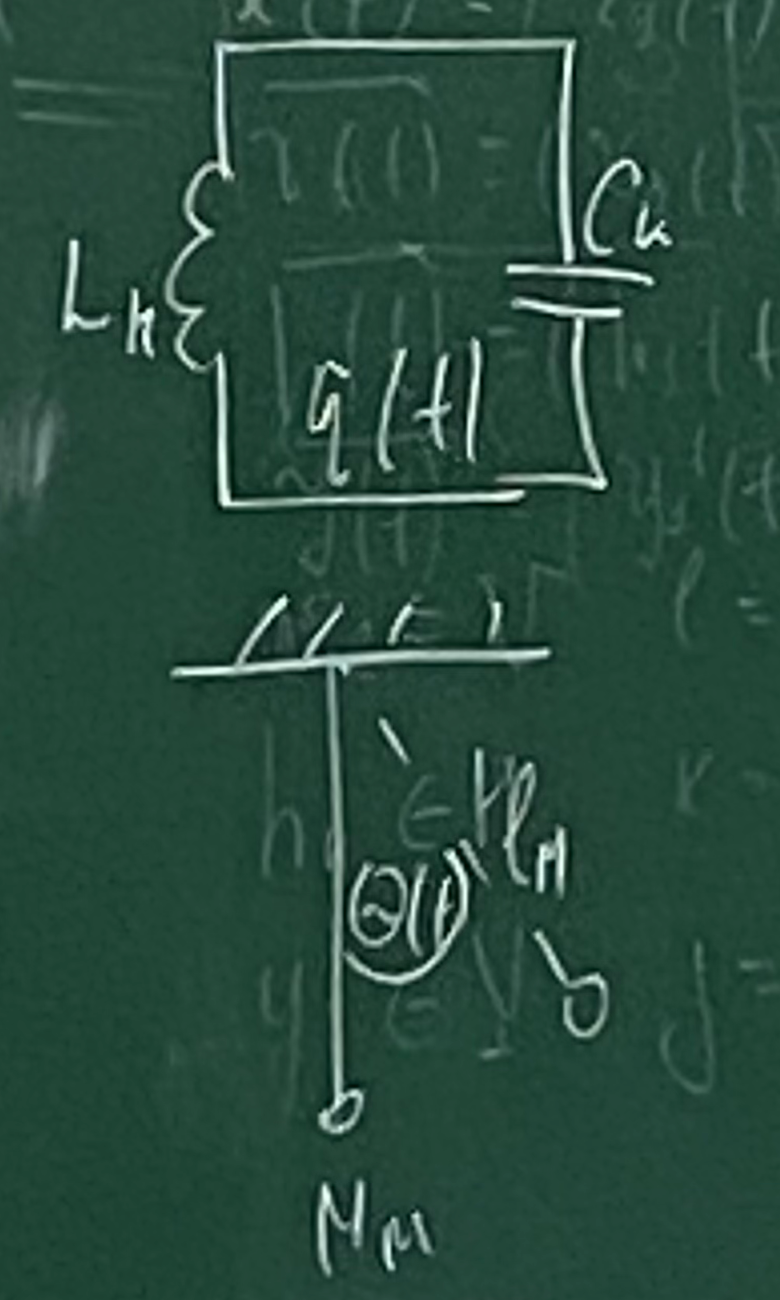
\includegraphics[width=0.3\textwidth]{img/content/06_types_schemes/example.png}
    \caption{Пример}
\end{figure}

Колебательный контур можно описать

\begin{equation*}
    L_k \frac{d^2 q(t)}{dt^2} + \frac{q(t)}{C_k} = 0
\end{equation*}

Маятник

\begin{equation*}
    m_m l_m^2 \frac{d^2 \Theta (t)}{dt^2} + m_m gl_m \Theta(t) = 0
\end{equation*}

\begin{equation*}
    h_2 \frac{d^2z(t)}{dt^2} + h_1 \frac{dz(t)}{dt} + h_0 z(t) = 0
\end{equation*}

В теории систем имеются базовые понятия:

\begin{itemize}
    \item \textbf{Система} -- множество элементов, находящихся в отношениях и связях между собой.
    \item \textbf{Элемент} -- часть системы, представление о которой нецелесообразно подвергать дальнейшему членению.
    \item \textbf{Сложная система} -- система, характеризуемая большим числом элементов и что наиболее важно большим числом взаимосвязей элементов. Сложность системы определяется так же видом взаимосвязей, свойствами, целенаправленности, целостностью, членимостью и иерархичностью, многоаспектностью.
    \item \textbf{Подсистема} -- часть системы (подмножество элементов и их взаимосвязей), которая имеет свойства системы.
    \item \textbf{Надсистема} -- система, по отношению к которой, рассматриваемая является подсистемой.
    \item \textbf{Структура} -- отображение совокупности элементов системы и их взаимосвязей. Отличается от понятия самой системы тем, что при описании структуры принимают во внимание лишь типы элементов и связей без конкретизации значений их параметров.
    \item \textbf{Параметр} -- величина, выражающая свойства или системы или ее части или влияющей на систему среды.
    \item \textbf{Целенаправленность} -- свойство искусственной системы, выражающее назначение системы, необходимой для оценки эффективности вариантов системы.
    \item \textbf{Целостность} -- свойство системы, характеризующая взаимосвязанность элементов и наличие зависимости выходных параметров от параметров элементов, при чем большинство выходных параметров не являются простым повторением или суммой параметров элементов.
    \item \textbf{Иерархичноть} -- важнейшее свойство сложной системы, выражающее возможность и целесообразность ее иерархического описания, то есть представление ее в виде нескольких уровней, между компонентами которых имеется отношение, целая часть.
\end{itemize}

2 четко различимые задачи:

\begin{itemize}
    \item modeling -- создание моделий
    \item simulating -- анализ свойств систем на основе исследования модели
\end{itemize}
